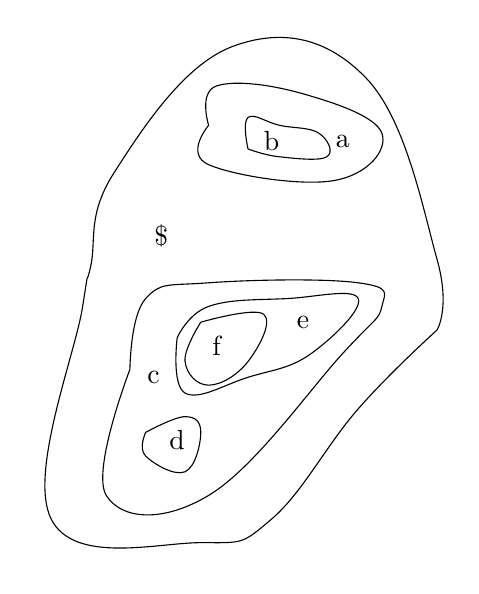
\begin{tikzpicture}

\draw  plot[smooth, tension=.7] coordinates {(0.3,0.5) (-0.7,-0.5) (-1.8,-1.9) (-2.7,-2.2) (-4.6,-1.9) (-4.2,0.8) (-4.1,1.3) (-3.8,2.5) (-2.3,4.1) (-0.6,3.7) (0.3,1.4) (0.3,0.5)};
\draw  plot[smooth, tension=.7] coordinates {(-2.7,0.6) (-2.9,0.1) (-2.6,-0.2) (-2.1,0.1) (-1.9,0.7) (-2.7,0.6)         };
\draw  plot[smooth, tension=.7] coordinates {(-3,0.4) (-2.6,0.8) (-1.6,0.9) (-0.7,0.9) (-1.3,0.2) (-2.1,-0.1) (-2.9,-0.3) (-3,0.4)};
\draw  plot[smooth, tension=.7] coordinates {(-3.6,0) (-3.4,0.9) (-2.6,1.1) (-0.7,1.1) (-0.4,0.8) (-0.9,0.2) (-2.6,-1.6) (-3.9,-1.6) (-3.6,0)};
\draw  plot[smooth, tension=.7] coordinates {(-3.4,-0.8) (-2.9,-0.6) (-2.7,-0.8) (-2.9,-1.3) (-3.4,-1.1) (-3.4,-0.8)};

\node at (-2.5,0.3) {f};
\node at (-1.4,0.6) {e};
\node at (-3,-0.9) {d};
\node at (-3.3,-0.1) {c};
\node at (-3.2,1.7) {$\$$};
\draw  plot[smooth, tension=.7] coordinates {(-2.1,2.8) (-2.1,3.2) (-1.7,3.1) (-1.2,3) (-1.1,2.7) (-1.7,2.7) (-2.1,2.8)};
\draw  plot[smooth, tension=.7] coordinates {(-2.6,3.1) (-2.5,3.6) (-1.4,3.5) (-0.4,3) (-1,2.4) (-2.6,2.6) (-2.6,3.1)};
\node at (-1.8,2.9) {b};
\node at (-0.9,2.9) {a};
\end{tikzpicture}